
%% bare_conf.tex
%% V1.4b
%% 2015/08/26
%% by Michael Shell
%% See:
%% http://www.michaelshell.org/
%% for current contact information.
%%
%% This is a skeleton file demonstrating the use of IEEEtran.cls
%% (requires IEEEtran.cls version 1.8b or later) with an IEEE
%% conference paper.
%%
%% Support sites:
%% http://www.michaelshell.org/tex/ieeetran/
%% http://www.ctan.org/pkg/ieeetran
%% and
%% http://www.ieee.org/

%%*************************************************************************
%% Legal Notice:
%% This code is offered as-is without any warranty either expressed or
%% implied; without even the implied warranty of MERCHANTABILITY or
%% FITNESS FOR A PARTICULAR PURPOSE! 
%% User assumes all risk.
%% In no event shall the IEEE or any contributor to this code be liable for
%% any damages or losses, including, but not limited to, incidental,
%% consequential, or any other damages, resulting from the use or misuse
%% of any information contained here.
%%
%% All comments are the opinions of their respective authors and are not
%% necessarily endorsed by the IEEE.
%%
%% This work is distributed under the LaTeX Project Public License (LPPL)
%% ( http://www.latex-project.org/ ) version 1.3, and may be freely used,
%% distributed and modified. A copy of the LPPL, version 1.3, is included
%% in the base LaTeX documentation of all distributions of LaTeX released
%% 2003/12/01 or later.
%% Retain all contribution notices and credits.
%% ** Modified files should be clearly indicated as such, including  **
%% ** renaming them and changing author support contact information. **
%%*************************************************************************


% *** Authors should verify (and, if needed, correct) their LaTeX system  ***
% *** with the testflow diagnostic prior to trusting their LaTeX platform ***
% *** with production work. The IEEE's font choices and paper sizes can   ***
% *** trigger bugs that do not appear when using other class files.       ***                          ***
% The testflow support page is at:
% http://www.michaelshell.org/tex/testflow/


\documentclass[conference,onecolumn,10pt]{IEEEtran}
\newtheorem{definition}{Definition}
% Some Computer Society conferences also require the compsoc mode option,
% but others use the standard conference format.
%
% If IEEEtran.cls has not been installed into the LaTeX system files,
% manually specify the path to it like:
% \documentclass[conference]{../sty/IEEEtran}

\usepackage{graphicx}
\usepackage{amsmath}
\usepackage{amssymb}
%\usepackage{subfig}
\usepackage{mathtools}
\usepackage{placeins}
%\usepackage[style=base]{caption}
\usepackage[caption=false]{subfig}
\usepackage[hyphens]{url}


% Some very useful LaTeX packages include:
% (uncomment the ones you want to load)


% *** MISC UTILITY PACKAGES ***
%
%\usepackage{ifpdf}
% Heiko Oberdiek's ifpdf.sty is very useful if you need conditional
% compilation based on whether the output is pdf or dvi.
% usage:
% \ifpdf
%   % pdf code
% \else
%   % dvi code
% \fi
% The latest version of ifpdf.sty can be obtained from:
% http://www.ctan.org/pkg/ifpdf
% Also, note that IEEEtran.cls V1.7 and later provides a builtin
% \ifCLASSINFOpdf conditional that works the same way.
% When switching from latex to pdflatex and vice-versa, the compiler may
% have to be run twice to clear warning/error messages.






% *** CITATION PACKAGES ***
%
%\usepackage{cite}
% cite.sty was written by Donald Arseneau
% V1.6 and later of IEEEtran pre-defines the format of the cite.sty package
% \cite{} output to follow that of the IEEE. Loading the cite package will
% result in citation numbers being automatically sorted and properly
% "compressed/ranged". e.g., [1], [9], [2], [7], [5], [6] without using
% cite.sty will become [1], [2], [5]--[7], [9] using cite.sty. cite.sty's
% \cite will automatically add leading space, if needed. Use cite.sty's
% noadjust option (cite.sty V3.8 and later) if you want to turn this off
% such as if a citation ever needs to be enclosed in parenthesis.
% cite.sty is already installed on most LaTeX systems. Be sure and use
% version 5.0 (2009-03-20) and later if using hyperref.sty.
% The latest version can be obtained at:
% http://www.ctan.org/pkg/cite
% The documentation is contained in the cite.sty file itself.






% *** GRAPHICS RELATED PACKAGES ***
%
\ifCLASSINFOpdf
  % \usepackage[pdftex]{graphicx}
  % declare the path(s) where your graphic files are
  % \graphicspath{{../pdf/}{../jpeg/}}
  % and their extensions so you won't have to specify these with
  % every instance of \includegraphics
  % \DeclareGraphicsExtensions{.pdf,.jpeg,.png}
\else
  % or other class option (dvipsone, dvipdf, if not using dvips). graphicx
  % will default to the driver specified in the system graphics.cfg if no
  % driver is specified.
  % \usepackage[dvips]{graphicx}
  % declare the path(s) where your graphic files are
  % \graphicspath{{../eps/}}
  % and their extensions so you won't have to specify these with
  % every instance of \includegraphics
  % \DeclareGraphicsExtensions{.eps}
\fi
% graphicx was written by David Carlisle and Sebastian Rahtz. It is
% required if you want graphics, photos, etc. graphicx.sty is already
% installed on most LaTeX systems. The latest version and documentation
% can be obtained at: 
% http://www.ctan.org/pkg/graphicx
% Another good source of documentation is "Using Imported Graphics in
% LaTeX2e" by Keith Reckdahl which can be found at:
% http://www.ctan.org/pkg/epslatex
%
% latex, and pdflatex in dvi mode, support graphics in encapsulated
% postscript (.eps) format. pdflatex in pdf mode supports graphics
% in .pdf, .jpeg, .png and .mps (metapost) formats. Users should ensure
% that all non-photo figures use a vector format (.eps, .pdf, .mps) and
% not a bitmapped formats (.jpeg, .png). The IEEE frowns on bitmapped formats
% which can result in "jaggedy"/blurry rendering of lines and letters as
% well as large increases in file sizes.
%
% You can find documentation about the pdfTeX application at:
% http://www.tug.org/applications/pdftex





% *** MATH PACKAGES ***
%
%\usepackage{amsmath}
% A popular package from the American Mathematical Society that provides
% many useful and powerful commands for dealing with mathematics.
%
% Note that the amsmath package sets \interdisplaylinepenalty to 10000
% thus preventing page breaks from occurring within multiline equations. Use:
%\interdisplaylinepenalty=2500
% after loading amsmath to restore such page breaks as IEEEtran.cls normally
% does. amsmath.sty is already installed on most LaTeX systems. The latest
% version and documentation can be obtained at:
% http://www.ctan.org/pkg/amsmath





% *** SPECIALIZED LIST PACKAGES ***
%
%\usepackage{algorithmic}
% algorithmic.sty was written by Peter Williams and Rogerio Brito.
% This package provides an algorithmic environment fo describing algorithms.
% You can use the algorithmic environment in-text or within a figure
% environment to provide for a floating algorithm. Do NOT use the algorithm
% floating environment provided by algorithm.sty (by the same authors) or
% algorithm2e.sty (by Christophe Fiorio) as the IEEE does not use dedicated
% algorithm float types and packages that provide these will not provide
% correct IEEE style captions. The latest version and documentation of
% algorithmic.sty can be obtained at:
% http://www.ctan.org/pkg/algorithms
% Also of interest may be the (relatively newer and more customizable)
% algorithmicx.sty package by Szasz Janos:
% http://www.ctan.org/pkg/algorithmicx




% *** ALIGNMENT PACKAGES ***
%
%\usepackage{array}
% Frank Mittelbach's and David Carlisle's array.sty patches and improves
% the standard LaTeX2e array and tabular environments to provide better
% appearance and additional user controls. As the default LaTeX2e table
% generation code is lacking to the point of almost being broken with
% respect to the quality of the end results, all users are strongly
% advised to use an enhanced (at the very least that provided by array.sty)
% set of table tools. array.sty is already installed on most systems. The
% latest version and documentation can be obtained at:
% http://www.ctan.org/pkg/array


% IEEEtran contains the IEEEeqnarray family of commands that can be used to
% generate multiline equations as well as matrices, tables, etc., of high
% quality.




% *** SUBFIGURE PACKAGES ***
%\ifCLASSOPTIONcompsoc
%  \usepackage[caption=false,font=normalsize,labelfont=sf,textfont=sf]{subfig}
%\else
%  \usepackage[caption=false,font=footnotesize]{subfig}
%\fi
% subfig.sty, written by Steven Douglas Cochran, is the modern replacement
% for subfigure.sty, the latter of which is no longer maintained and is
% incompatible with some LaTeX packages including fixltx2e. However,
% subfig.sty requires and automatically loads Axel Sommerfeldt's caption.sty
% which will override IEEEtran.cls' handling of captions and this will result
% in non-IEEE style figure/table captions. To prevent this problem, be sure
% and invoke subfig.sty's "caption=false" package option (available since
% subfig.sty version 1.3, 2005/06/28) as this is will preserve IEEEtran.cls
% handling of captions.
% Note that the Computer Society format requires a larger sans serif font
% than the serif footnote size font used in traditional IEEE formatting
% and thus the need to invoke different subfig.sty package options depending
% on whether compsoc mode has been enabled.
%
% The latest version and documentation of subfig.sty can be obtained at:
% http://www.ctan.org/pkg/subfig




% *** FLOAT PACKAGES ***
%
%\usepackage{fixltx2e}
% fixltx2e, the successor to the earlier fix2col.sty, was written by
% Frank Mittelbach and David Carlisle. This package corrects a few problems
% in the LaTeX2e kernel, the most notable of which is that in current
% LaTeX2e releases, the ordering of single and double column floats is not
% guaranteed to be preserved. Thus, an unpatched LaTeX2e can allow a
% single column figure to be placed prior to an earlier double column
% figure.
% Be aware that LaTeX2e kernels dated 2015 and later have fixltx2e.sty's
% corrections already built into the system in which case a warning will
% be issued if an attempt is made to load fixltx2e.sty as it is no longer
% needed.
% The latest version and documentation can be found at:
% http://www.ctan.org/pkg/fixltx2e


%\usepackage{stfloats}
% stfloats.sty was written by Sigitas Tolusis. This package gives LaTeX2e
% the ability to do double column floats at the bottom of the page as well
% as the top. (e.g., "\begin{figure*}[!b]" is not normally possible in
% LaTeX2e). It also provides a command:
%\fnbelowfloat
% to enable the placement of footnotes below bottom floats (the standard
% LaTeX2e kernel puts them above bottom floats). This is an invasive package
% which rewrites many portions of the LaTeX2e float routines. It may not work
% with other packages that modify the LaTeX2e float routines. The latest
% version and documentation can be obtained at:
% http://www.ctan.org/pkg/stfloats
% Do not use the stfloats baselinefloat ability as the IEEE does not allow
% \baselineskip to stretch. Authors submitting work to the IEEE should note
% that the IEEE rarely uses double column equations and that authors should try
% to avoid such use. Do not be tempted to use the cuted.sty or midfloat.sty
% packages (also by Sigitas Tolusis) as the IEEE does not format its papers in
% such ways.
% Do not attempt to use stfloats with fixltx2e as they are incompatible.
% Instead, use Morten Hogholm'a dblfloatfix which combines the features
% of both fixltx2e and stfloats:
%
% \usepackage{dblfloatfix}
% The latest version can be found at:
% http://www.ctan.org/pkg/dblfloatfix




% *** PDF, URL AND HYPERLINK PACKAGES ***
%
%\usepackage{url}
% url.sty was written by Donald Arseneau. It provides better support for
% handling and breaking URLs. url.sty is already installed on most LaTeX
% systems. The latest version and documentation can be obtained at:
% http://www.ctan.org/pkg/url
% Basically, \url{my_url_here}.




% *** Do not adjust lengths that control margins, column widths, etc. ***
% *** Do not use packages that alter fonts (such as pslatex).         ***
% There should be no need to do such things with IEEEtran.cls V1.6 and later.
% (Unless specifically asked to do so by the journal or conference you plan
% to submit to, of course. )


% correct bad hyphenation here
\hyphenation{op-tical net-works semi-conduc-tor}


\begin{document}
%
% paper title
% Titles are generally capitalized except for words such as a, an, and, as,
% at, but, by, for, in, nor, of, on, or, the, to and up, which are usually
% not capitalized unless they are the first or last word of the title.
% Linebreaks \\ can be used within to get better formatting as desired.
% Do not put math or special symbols in the title.
\title{Trajectory Generation and Control for Quadrotors}


% author names and affiliations
% use a multiple column layout for up to three different
% affiliations
\author{\IEEEauthorblockN{Sandesh Thapa}
\IEEEauthorblockA{MAE/ECEN 5473 Digital Control Systems\\School of Mechanical and Aerospace Engineering\\
Oklahoma State University\\
Stillwater, Oklahoma\\
Email: sandesh.thapa@okstate.edu}}
%\and
%\IEEEauthorblockN{Homer Simpson}
%\IEEEauthorblockA{Twentieth Century Fox\\
%Springfield, USA\\
%Email: homer@thesimpsons.com}
%\and
%\IEEEauthorblockN{James Kirk\\ and Montgomery Scott}
%\IEEEauthorblockA{Starfleet Academy\\
%San Francisco, California 96678--2391\\
%Telephone: (800) 555--1212\\
%Fax: (888) 555--1212}}

% conference papers do not typically use \thanks and this command
% is locked out in conference mode. If really needed, such as for
% the acknowledgment of grants, issue a \IEEEoverridecommandlockouts
% after \documentclass

% for over three affiliations, or if they all won't fit within the width
% of the page, use this alternative format:
% 
%\author{\IEEEauthorblockN{Michael Shell\IEEEauthorrefmark{1},
%Homer Simpson\IEEEauthorrefmark{2},
%James Kirk\IEEEauthorrefmark{3}, 
%Montgomery Scott\IEEEauthorrefmark{3} and
%Eldon Tyrell\IEEEauthorrefmark{4}}
%\IEEEauthorblockA{\IEEEauthorrefmark{1}School of Electrical and Computer Engineering\\
%Georgia Institute of Technology,
%Atlanta, Georgia 30332--0250\\ Email: see http://www.michaelshell.org/contact.html}
%\IEEEauthorblockA{\IEEEauthorrefmark{2}Twentieth Century Fox, Springfield, USA\\
%Email: homer@thesimpsons.com}
%\IEEEauthorblockA{\IEEEauthorrefmark{3}Starfleet Academy, San Francisco, California 96678-2391\\
%Telephone: (800) 555--1212, Fax: (888) 555--1212}
%\IEEEauthorblockA{\IEEEauthorrefmark{4}Tyrell Inc., 123 Replicant Street, Los Angeles, California 90210--4321}}




% use for special paper notices
%\IEEEspecialpapernotice{(Invited Paper)}




% make the title area
\maketitle

% As a general rule, do not put math, special symbols or citations
% in the abstract
\begin{abstract}

In this project, I explored the controller design and trajectory generation for quadrotor. Differential flatness was used for trajectory generation based on the one of the references. Minimum snap trajectory is generated from the given algorithm based on waypoints navigation and a simple proportional plus derivative (PD)controller is used to track the trajectories. Simulations results are presented which generates smooth trajectories for position and velocity of the quadrotor.



\end{abstract}

% no keywords




% For peer review papers, you can put extra information on the cover
% page as needed:
% \ifCLASSOPTIONpeerreview
% \begin{center} \bfseries EDICS Category: 3-BBND \end{center}
% \fi
%
% For peerreview papers, this IEEEtran command inserts a page break and
% creates the second title. It will be ignored for other modes.
\IEEEpeerreviewmaketitle



\section{Introduction}
Recently, quadrotors are being widely used for research. Because of it's agility in 3D Euclidean space, it can be used for variety of purpose including photography, inspection, transportation of loads, geo-surveying and so on. For a quadrotor maneuvering in tightly constraint environment, it is necessary to develop optimal trajectories to ensure safe passage through corridors and constraints \cite{mellinger2011minimum}. So, it is necessary to develop flight plans that leverage the dynamics of system \cite{mellinger2011minimum}.




% An example of a floating figure using the graphicx package.
% Note that \label must occur AFTER (or within) \caption.
% For figures, \caption should occur after the \includegraphics.
% Note that IEEEtran v1.7 and later has special internal code that
% is designed to preserve the operation of \label within \caption
% even when the captionsoff option is in effect. However, because
% of issues like this, it may be the safest practice to put all your
% \label just after \caption rather than within \caption{}.
%
% Reminder: the "draftcls" or "draftclsnofoot", not "draft", class
% option should be used if it is desired that the figures are to be
% displayed while in draft mode.
%
%\begin{figure}[!t]
%\centering
%\includegraphics[width=2.5in]{myfigure}
% where an .eps filename suffix will be assumed under latex, 
% and a .pdf suffix will be assumed for pdflatex; or what has been declared
% via \DeclareGraphicsExtensions.
%\caption{Simulation results for the network.}
%\label{fig_sim}
%\end{figure}

% Note that the IEEE typically puts floats only at the top, even when this
% results in a large percentage of a column being occupied by floats.


% An example of a double column floating figure using two subfigures.
% (The subfig.sty package must be loaded for this to work.)
% The subfigure \label commands are set within each subfloat command,
% and the \label for the overall figure must come after \caption.
% \hfil is used as a separator to get equal spacing.
% Watch out that the combined width of all the subfigures on a 
% line do not exceed the text width or a line break will occur.
%
%\begin{figure*}[!t]
%\centering
%\subfloat[Case I]{\includegraphics[width=2.5in]{box}%
%\label{fig_first_case}}
%\hfil
%\subfloat[Case II]{\includegraphics[width=2.5in]{box}%
%\label{fig_second_case}}
%\caption{Simulation results for the network.}
%\label{fig_sim}
%\end{figure*}
%
% Note that often IEEE papers with subfigures do not employ subfigure
% captions (using the optional argument to \subfloat[]), but instead will
% reference/describe all of them (a), (b), etc., within the main caption.
% Be aware that for subfig.sty to generate the (a), (b), etc., subfigure
% labels, the optional argument to \subfloat must be present. If a
% subcaption is not desired, just leave its contents blank,
% e.g., \subfloat[].


% An example of a floating table. Note that, for IEEE style tables, the
% \caption command should come BEFORE the table and, given that table
% captions serve much like titles, are usually capitalized except for words
% such as a, an, and, as, at, but, by, for, in, nor, of, on, or, the, to
% and up, which are usually not capitalized unless they are the first or
% last word of the caption. Table text will default to \footnotesize as
% the IEEE normally uses this smaller font for tables.
% The \label must come after \caption as always.
%
%\begin{table}[!t]
%% increase table row spacing, adjust to taste
%\renewcommand{\arraystretch}{1.3}
% if using array.sty, it might be a good idea to tweak the value of
% \extrarowheight as needed to properly center the text within the cells
%\caption{An Example of a Table}
%\label{table_example}
%\centering
%% Some packages, such as MDW tools, offer better commands for making tables
%% than the plain LaTeX2e tabular which is used here.
%\begin{tabular}{|c||c|}
%\hline
%One & Two\\
%\hline
%Three & Four\\
%\hline
%\end{tabular}
%\end{table}


% Note that the IEEE does not put floats in the very first column
% - or typically anywhere on the first page for that matter. Also,
% in-text middle ("here") positioning is typically not used, but it
% is allowed and encouraged for Computer Society conferences (but
% not Computer Society journals). Most IEEE journals/conferences use
% top floats exclusively. 
% Note that, LaTeX2e, unlike IEEE journals/conferences, places
% footnotes above bottom floats. This can be corrected via the
% \fnbelowfloat command of the stfloats package.

\section{Project Objective}
The objective of this project is to review and develop understanding of trajectory generation for quadrotors. I reviewed \cite{mellinger2011minimum} and related sources \cite{mellinger2012trajectory, michael2010grasp} to understand and implement differential flatness for trajectory generation Examples code were given at \cite{AerialRobotics, AerialRobotics1}. I implemented Mellinger's minimum snap trajectory and control algorithm for quadrotors based on differential flatness \cite{mellinger2011minimum, mellinger2012trajectory}. The goal of the this project was to develop a strong understanding of quadrotor trajectory generation and control algorithm so that it can be applied to mutliagents path planning and control problems in future works. 
\section{Methodology}
In this paper, I used the dynamic model and control from \cite{mellinger2011minimum} and implemented in MATLAB. I used a PD controller to track a given trajectory. Trajectories are generated based differential flatness which ensures smoothness. I compared minimum snap trajectory and shortest distance trajectory and distinguished their performance. 

\section{Dynamic Model}
\begin{figure}[h!]
\centering
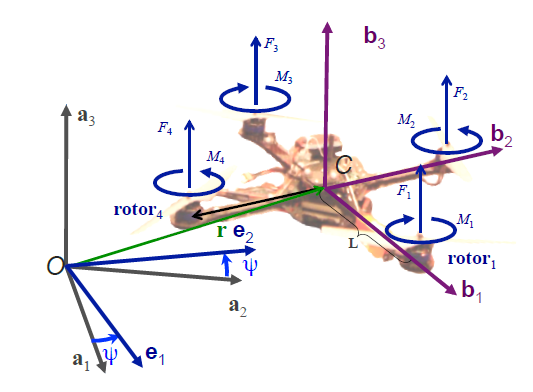
\includegraphics[scale=0.4]{images/Quadmodel.png}
\caption{Quadrotor model with the body-fixed and inertial reference frames.}
\label{Quadmodel}
\end{figure}
\subsection{Coordinate Systems}
The coordinate systems with a free body diagram for the quadrotor is shown in Fig.~\ref{Quadmodel}. $\mathcal{A}$ is the inertial frame with axis $\mathsf{a}_1$, $\mathsf{a}_2$ and $\mathsf{a}_3$. The body frame $\mathcal{B}$, is attached to the center of mass of the quadrotor which is coincident with the inertial frame. $\mathcal{C}$ is the center mass of the rotor and ${L}$ is the length of the rotors from the center $\mathcal{C}$

\subsection{Motor Model}
Each rotor has an angular speed $\omega_i$ and produces a vertical force $F_i$, which is given by 
\begin{equation}
\label{Fi}
F_i = k_F\omega_i^2,
\end{equation}
$k_F \approx 6.11\times10^{-8} \frac{N}{rmp^2}$ \cite{michael2010grasp}.
\begin{equation}
\label{Mi}
M_i = k_M\omega_i^2,
\end{equation}
$k_M \approx 1.5\times10^{-9} \frac{Nm}{rmp^2}$ \cite{michael2010grasp}.
\subsection{Rigid Body Dynamics}
The orientation of quadrotor is described by triplet of yaw-pitch-roll($\phi$, $\theta$ and $\psi$) $Z-Y-X$ Euler angles. The position of center of mass of quadrotor is given by 
\begin{equation}
\textbf{r} = \begin{bmatrix}
x&y&z
\end{bmatrix}^T.
\end{equation}
The state of the quadrotor is given by 
\begin{equation}
q = \begin{bmatrix}
x & y & z & \phi & \theta & \psi 
\end{bmatrix}^T.
\end{equation}
The rotation matrix from $\mathcal{B}$ to $\mathcal{A}$ is given by, 
\begin{equation}
\label{Rot}
R_{BA} = \begin{bmatrix}
c\phi c\theta-s\phi s\psi s\theta & -c\phi s\psi & c\psi s\theta + c \theta s \phi s \psi \\
c \theta s \psi + c \psi s \phi s \theta & c \phi c \psi & s \psi s \theta -c \psi c \theta s \phi \\
-c \phi s \theta & s \phi & c \phi c \theta 
\end{bmatrix}.
 \end{equation}
 The angular velocity of the robot in the body frame is denoted as $q$, $q$ and $r$. These values are related to derivatives of the roll, pitch and yaw angles according to 
 \begin{equation}
 \label{pqr}
 \begin{bmatrix}
 p\\
 q\\
 r\\
 \end{bmatrix} = \begin{bmatrix}
 c\theta & 0 & -c\phi s \theta \\
 0 & 1 & s \phi \\
 s \theta & 0 & c \phi c \theta 
 \end{bmatrix} \begin{bmatrix}
 \dot{\phi}\\
 \dot{\theta}\\
 \dot{\psi}
 \end{bmatrix}.
 \end{equation}

\subsubsection{Newton's Equations of Motion}
The force in the system are gravity, and the forces from each rotors $F_i$. The equation governing the acceleration of center of mass of quadrotor is 
\begin{equation}
\label{nweq}
m\ddot{\textbf{r}} = \begin{bmatrix}
0 \\
0\\
mg \\
\end{bmatrix} + R_{BA} \begin{bmatrix}
0 \\
0\\
F_1 + F_2 + F_3 + F_4
\end{bmatrix},
\end{equation}
The first input to the system $u_1$ is defined as 
$$u_1 = \sum_{i=1}^4F_i$$.
\subsubsection{Euler's Equations of Motion}
In addition to forces, each rotor produces a moment perpendicular to the plan to rotation of the blade, $M_i$. Rotors 1 and 3 rotate in the $-\mathsf{b}_3$ direction while 2 and 4 rotate in the $+\mathsf{b}_3$ direction. The moment produced on the quadrotor is opposite to the direction of rotation of the blades. So, $M_1$ and $M_3$ act in the $\mathsf{b}_3$ direction while $M_2$ and $M_4$ act in the $-\mathsf{b}_3$ direction. The angular acceleration is determined by, 
\begin{equation}
\label{ELEq}
I\begin{bmatrix}
\dot{p}\\
\dot{q} \\
\dot{r}
\end{bmatrix} = \begin{bmatrix}
L(F_2-F_4) \\
L(F_3-F_1)\\
M_1-M_2+M_3-M_4
\end{bmatrix} - \begin{bmatrix}
p\\
q\\
r\\
\end{bmatrix}\times I  \begin{bmatrix}
p\\
q\\
r\\
\end{bmatrix}.
\end{equation}
We can rewrite this as: 
\begin{equation}
\label{ELEq}
I\begin{bmatrix}
\dot{p}\\
\dot{q} \\
\dot{r}
\end{bmatrix} = \begin{bmatrix}
0 & L & 0 & -L \\
-L & 0 & L & 0 \\
\gamma & -\gamma & \gamma & -\gamma
\end{bmatrix}\begin{bmatrix}
F_1\\
F_2\\
F_3\\
F_4 \\
\end{bmatrix} - \begin{bmatrix}
p\\
q\\
r\\
\end{bmatrix}\times I  \begin{bmatrix}
p\\
q\\
r\\
\end{bmatrix},
\end{equation}
where $\gamma = \frac{k_M}{k_F}$. Second input  $\textbf{u}_2$ is defined as: $$ \textbf{u}_2 = 
\begin{bmatrix}
0 & L & 0 & -L \\
-L & 0 & L & 0 \\
\gamma & -\gamma & \gamma & -\gamma
\end{bmatrix}  \begin{bmatrix}
F_1\\
F_2\\
F_3\\
F_4 \\
\end{bmatrix}.$$

\section{Control}
The controller used in \cite{mellinger2011minimum, michael2010grasp} are derived by linearizing the equation of motion about an operating point, $\textbf{r} = \textbf{r}_0$, $\theta = \phi = 0$, $\psi = \psi_0$, $\dot{\textbf{r}} = 0$, and $\dot{\phi}= \dot{\theta} = \dot{\psi} = 0$. Using small angle approximation for roll and pitch angles ($c\phi = 1$, $c\theta = 1$, $s\phi \approx \phi$, and $s\theta \approx \theta$) gives use the following linearized equations:
\begin{equation}
F_{i,0} = \frac{mg}{4},
\end{equation}
At nominal state, the inputs for hover are $u_{1,0} = mg$, $\textbf{u}_{2,0} = 0$.

Linearizing \eqref{nweq}, we get: 
\begin{equation}
\begin{aligned}
\label{rddot}
\ddot{r}_1 &= g(\Delta\theta \cos \psi_0 + \Delta \phi \sin \psi_0) \\
\ddot{r}_2 &= g(\Delta\theta \sin \psi_0 - \Delta \phi \cos \psi_0) \\
\ddot{r}_3 &= \frac{1}{m}u_1 - g
\end{aligned}
\end{equation}
Linearizing \eqref{ELEq}, we get: 
\begin{equation}
\label{pqrddot} 
\begin{bmatrix}
\dot{p} \\
\dot{q}\\
\dot{r} \\
\end{bmatrix} = I^{-1}
\begin{bmatrix}
0 & L & 0 & -L \\
-L & 0 & L & 0 \\
\gamma & -\gamma & \gamma & -\gamma
\end{bmatrix}  \begin{bmatrix}
F_1\\
F_2\\
F_3\\
F_4 \\
\end{bmatrix}
\end{equation}
The rotor cart is assumed to be symmetric so $I_{xx} = I_{yy}$, 
\begin{equation}
\begin{aligned}
\dot{p} &= \frac{u_{2,x}}{I_{xx}} = \frac{L}{I_{xx}}(F_2-F_4)\\
\dot{q} &= \frac{u_{2,y}}{I_{yy}} = \frac{L}{I_{yy}}(F_3-F_1)\\
\dot{r} &= \frac{u_{2,z}}{I_{zz}} = \frac{\gamma}{I_{zz}}(F_1-F_2+F_3-F_4)
\end{aligned}
\end{equation}
\subsection{Position and Attitude Controller}
\begin{figure}[h!]
\centering
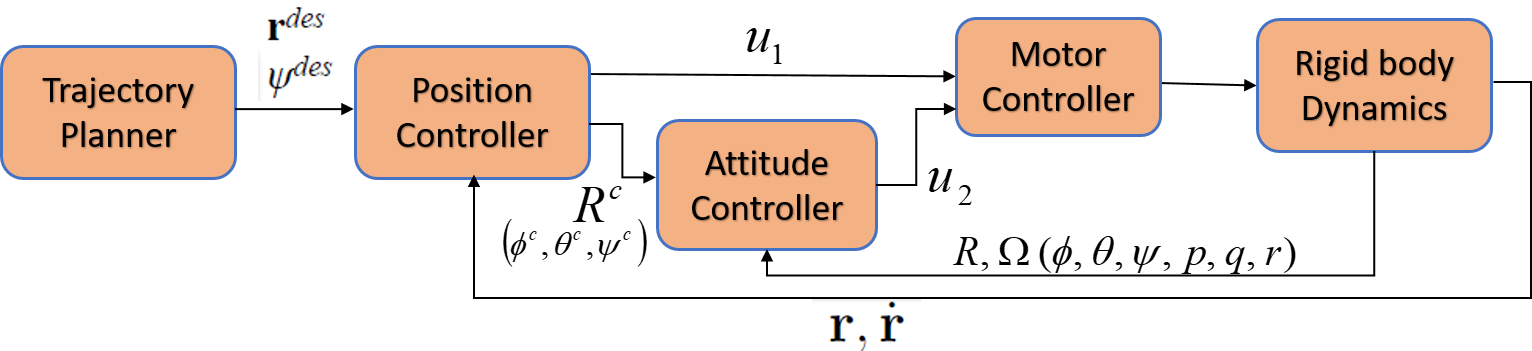
\includegraphics[scale=0.5]{images/controlmy2.png}
\caption{The position and attitude control loops.}
\label{Control1}
\end{figure}

The control problem is to determine the four inputs, ($u_1, \textbf{u}_2$) required to hover or to follow a desired trajectory, $\textbf{z}_des$. As shown in Fig. \ref{Control1}, error in the robot's position is used to derive the controller from \eqref{rddot} The equations in \eqref{rddot} also allows us to derive a desired orientation. The attitude controller for this desired orientation is derived from \eqref{pqrddot}. We require the attitude control loop to run in a higher rate than the position control loop. 
\subsubsection{Attitude Control} 
Mellinger \cite{mellinger2011minimum} develop a following PD controller for attitude control:
\begin{equation}
\label{attitudeC}
\textbf{u}_2 = \begin{bmatrix}
k_{p,\phi}(\phi_{des} - \phi)+ k_{d,\phi}(p_{des}-p) \\
k_{p,\theta}(\theta_{des} - \theta)+ k_{d,\theta}(q_{des}-q) \\
k_{p,\psi}(\psi_{des} - \psi)+ k_{d,\psi}(r_{des}-r)
\end{bmatrix}.
\end{equation}
here, $k_{p,i} \quad \text{and} \quad k_{d,i}$ are the control gains that needs to be tuned.
\subsubsection{Position Control} 
If a desired trajectory is given as: $$\textbf{z}_des = \begin{bmatrix}
\textbf{r}_{des}(t) \\
\psi_T(t)
\end{bmatrix},$$
following PD control is used to track  the yaw angles and 3 position of the rotor. 
\begin{equation}
\ddot{r}_{i,c} = \ddot{r}_{i,des} + k_{d,i}(\dot{r}_{i,des} - \dot{r}_i ) + k_{p,i}(r_{i,des}-r_i).
\end{equation}
%From \eqref{rddot} we can obtain the relationship between the desired acceleration, roll and pitch angles($\Delta \theta = \theta - \theta_0$ and $\Delta \phi = \phi_0$). 
%\begin{equation}
%\label{desrddot}
%\begin{aligned}
%\ddot{r}_{1,des} &= g(\theta_{des}\cos \psi_T + \phi_des \sin \psi_T) \\
%\ddot{r}_{2,des} &= g(\theta_{des}\sin \psi_T + \phi_des \cos \psi_T) \\
%\ddot{r}_{3,des}  &=  \frac{1}{m}u_1 - g
%\end{aligned}
%\end{equation}
which gives us 
\begin{equation}
\label{desddt}
u_1 = m(g+\ddot{r}_{3,c}).
\end{equation}

we find the desired roll and pitch angles as 
\begin{equation}
\begin{aligned}
\phi_{des} &= \frac{1}{g}(\ddot{r}_{1,c}\sin \psi_{des} - \ddot{r}_{2,c}\cos \psi_{des} ), \\
\theta_{des} &= \frac{1}{g}(\ddot{r}_{1,c}\cos \psi_{des} + \ddot{r}_{2,c}\sin \psi_{des}. )
\end{aligned}
\end{equation}
The desired roll and pitch velocities are taken to be zero.
\section{Differential Flatness}
\begin{definition}
A nonlinear system 
\begin{equation}
\label{xdot}
\begin{aligned}
\dot{x} &= f(x,u), & x \in \mathbb{R}^n, & \quad u \in \mathbb{R}^m,\\
y &= h(x),   & y \in \mathbb{R}^m, &
\end{aligned}
\end{equation}
\end{definition}
is differentially flat if we can find outputs $z \in \mathbb{R}^m$ of the form 
\begin{equation}
\label{z}
z \ \zeta(x,u,\dot{u},...,u^{(l)}),
\end{equation} 
such that 
\begin{equation}
\begin{aligned}
x &= x(z ,\dot{z}, ...,z^{(l)} \coloneqq x(\bar{z}),\\
u &= u(z,\dot{z},...,z^{(l)}) \coloneqq u(\bar{z}).
\end{aligned}
\end{equation}
A non linear system is differentially flat if we can find a set of outputs such that we can express all states and inputs in terms of those outputs and their derivatives \cite{van1997real}. 
\subsection{Example}
\begin{figure}[h!]
\centering
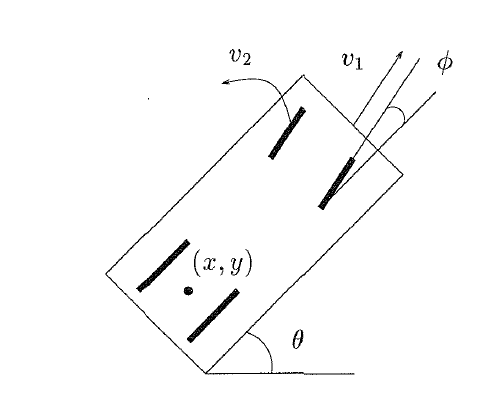
\includegraphics[scale=0.4]{images/car.png}
\caption{Kinematic Car}
\label{Car}
\end{figure}
A kinematic car is differentially flat system as whown in \cite{van1997trajectory} \\
Equations of motion 
\begin{equation}
\begin{aligned}
\dot{x} &= \cos \theta \cos \phi v_1 \\
\dot{y} &= \sin \theta \cos \phi v_2 \\
\dot{\theta} &= \frac{1}{l}\sin \phi v_1 \\
\phi &= v_2
\end{aligned}
\end{equation}
where, $v_1$ and $v_2$ are the inputs of the system.
If output is chosen to be $(x, y)$, $\phi$ can be expressed in terms of flat outputs as 
\begin{equation}
\phi \arctan (\frac{1}{l}({\dot{x}^2+\dot{y}^2)}^{\frac{3}{2}},\dot{x}\ddot{x}-\dot{y}\ddot{y}),
\end{equation}
which shows that kinematic car is differentially flat system.
\subsection{Quadrotor a Differentially Flat System}
From \eqref{nweq}, we get 
\begin{equation}
\label{nweq2}
m\ddot{\textbf{r}} = \begin{bmatrix}
0 \\
0\\
mg \\
\end{bmatrix} + R_{BA} \begin{bmatrix}
0 \\
0\\
u_1
\end{bmatrix}
\end{equation}
Using linearized equation of motions near hover assuming small angle assumptions we get, 
\begin{equation}
\label{Dfu1}
\begin{aligned}
m\ddot{x} &= (\theta c \psi + \phi s \psi)u_1 \\
m\ddot{y} &= (\theta s \psi - \phi c \psi)u_1 \\
m\ddot{z} &= -mg + u_1
\end{aligned}
\end{equation}
It shows the second derivative of position is proportional to input $u_1$. 

From the angular rate equation \eqref{pqr}, we get:
\begin{equation}
\label{DFu2}
\begin{aligned}
p &= \dot{\phi}c\theta - \dot{\psi}c \phi s \theta  \\
q & = \dot{\theta} + \dot{\psi}s \phi \\
r & = \dot{\phi} s \theta + \dot{\psi}c\phi c \theta 
\end{aligned}
\end{equation} 
Substituting the approximation:

$\sin(\theta) \approx \theta, \sin(\phi) \approx \phi, \cos(\phi) = \cos(\theta) \approx 1$, we get:
\begin{equation}
\label{DFu2qpqr}
\begin{aligned}
p &= \dot{\phi} - \dot{\psi} \theta  \\
q & = \dot{\theta} + \dot{\psi}\phi \\
r & = \dot{\phi} \theta + \dot{\psi}
\end{aligned}
\end{equation}
Further substituting: 

$\dot{\psi} \theta \approx \dot{\psi}\phi \approx \dot{\phi} \theta  = 0  $, 
we get: 
\begin{equation}
\label{jpayetehi}
\begin{aligned}
p = \dot{\phi} \\
q = \dot{\theta} \\
r = \dot{\psi}
\end{aligned}
\end{equation}
Now only considering the principal axis for inertia of the quadrotor and using \eqref{ELEq}, we get: 
\begin{equation}
\label{bigeqn}
\begin{bmatrix}
I_{xx} & 0 & 0\\
0 & I_{yy} & 0 \\
0 & 0 & I_{zz} \\
\end{bmatrix} \begin{bmatrix}
\dot{q} \\
\dot{q} \\
\dot{r} \\ 
\end{bmatrix} = \begin{bmatrix}
u_{2,x} \\
u_{2,y} \\
u_{2,z} \\
\end{bmatrix} - \begin{bmatrix}
0 & r & -q\\
-r& 0 & p \\
 q & -p & 0 \\
\end{bmatrix} \begin{bmatrix}
I_{xx} & 0 & 0\\
0 & I_{yy} & 0 \\
0 & 0 & I_{zz} \\
\end{bmatrix} \begin{bmatrix}
p \\
q \\
r \\
\end{bmatrix}
\end{equation}
From \eqref{bigeqn}, we get: 
\begin{equation}
\begin{aligned}
I_{xx}\dot{p} & = u_{2,x} - I_{yy}qr + I_{zz} qr \\ 
I_{yy}\dot{q} & = u_{2,y} + I_{xx}pr - I_{zz} pr \\
I_{xx}\dot{r} & = u_{2,z} - I_{xx}pq + I_{zz} pq \\
\end{aligned}
\end{equation}

Using approximation, $\dot{\psi} \dot{\theta} \approx \dot{\psi}\dot{\phi} \approx \dot{\phi} \dot{\theta} = pq = pr = qr = 0   $,
\begin{equation}
\label{eqn:mm}
\begin{aligned}
I_{xx}\dot{p} & = u_{2,x}  \\ 
I_{yy}\dot{q} & = u_{2,y}  \\
I_{xx}\dot{r} & = u_{2,z} \\
\end{aligned}
\end{equation}

From \eqref{jpayetehi} and \eqref{muji}, we get : 
\begin{equation}
\label{muji}
\begin{aligned}
\ddot{\phi} & = \frac{u_{2,x}}{I_{xx}} \\ 
\ddot{\theta} &= \frac{u_{2,y}}{I_{yy}}  \\
\ddot{\psi} & = \frac{u_{2,z}}{ I_{xx}}
\end{aligned}
\end{equation}
Differentiating \eqref{Dfu1}, 
\begin{equation}
\label{lamo}
\dddot{x} = \Big(\theta c \psi + \phi s \psi)\Big)\dot{u_1}+ \Big(\dot{\theta} c \psi -\thetas\psi \dot{\psi} + \dot{\phi} s \psi + \phi c \psi \dot{\psi}\Big){u_1}
\end{equation}

Differentiating again,

 \begin{equation}
\label{lamo}
\ddddot{x} = \Big(\theta c \psi + \phi s \psi)\Big)\ddot{u_1}+ 2\Big(\dot{\theta} c \psi -\thetas\psi \dot{\psi} + \dot{\phi} s \psi + \phi c \psi \dot{\psi}\Big)\dot{u_1} + \\
\Big(\ddot{\theta}c\psi -\dot{\theta}s \psi \dot{\psi} - \theta s \psi \ddot{\psi}  - \theta s \psi \dot{\psi}^2 + \ddot{\phi}s \psi + \dot{\phi} c \psi \dot{\psi} +  \dot{\phi} c \psi \ddot{\psi} - \dot{\phi} c \psi \dot{\psi}^2 \Big)u_1
\end{equation}
%
After substituting $\ddddot{x}$ into \eqref{eqn:mm}, we can prove that the fourth derivative of position is proportional to $u_2$. So,it is proved that quadrotor is a differentially flat system \cite{mellinger2011minimum} \cite{AerialRobotics}. 

\section{3D Trajectory Generation} 
For the purpose of this simulation, I used the optimal trajectory defined in  \cite{mellinger2011minimum} 
For optimal trajectory following function is used based on Calculus of Variations, 
\begin{equation}
\label{opt}
x*(t) = arg \min_{x(t)} \int_0^TL(\dot{x},xt)dt
\end{equation}
Solving functional $L$ using Euler-Lagrange equation gives use the optimal function. 
\begin{equation}
{d}{dt}\Big(\frac{\partial L}{\partial \dot{x}}\Big) - \frac{\partial L}{\partial {x}} = 0 
\end{equation}

For smooth trajectories generation, Mellinger \cite{mellinger2011minimum}, use following functional 
\begin{equation}
\label{opt}
x*(t) = arg \min_{x(t)} \int_0^T(({x^n})^2)dt
\end{equation}
when n = 1, we get shortest distance with minimum velocity, n = 2 gives minimum acceleration, n = 3 gives minimum acceleration and n = 4 produces minimum snap trajectory. For rest of the paper, I will be using minimum snap trajectory for simulation purpose. 

\subsection{Minimum Snap Trajectory}

%\begin{figure}[h!]
%\centering
%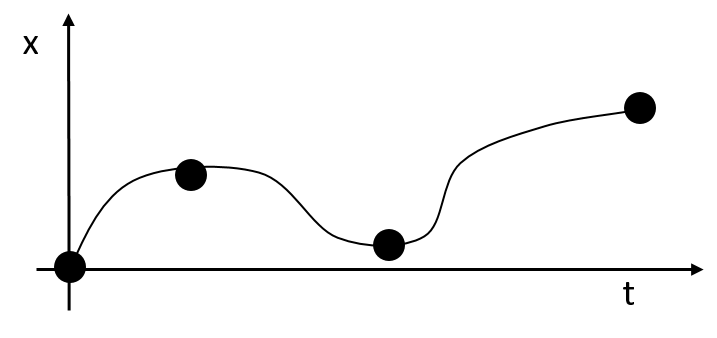
\includegraphics[scale=0.5]{images/traj.png}
%\caption{Kinematic Car}
%\label{Car}
%\end{figure}
Minimum snap trajectory is 7th order polynomial of time \cite{AerialRobotics}, \cite{mellinger2011minimum}. If we are given a set of $n+1$ waypoints $w_0,...w_n$, the minimum snap trajectory is a piecewise polynomial composed of $n$ 7th order polynomials. Each polynomial piece $p_i$ travels between a pair of waypoints $w_{i-1}$ and $w_i$ and takes a known amount of time $T_i$ to complete $i = 1,...,n$. 

Let $S_0 = 0$ and for $i = 1,...,n, S_i = \sum_{k=1}^{i}T_k$. $S_i$ is the time it takes to reach waypoint $w_i$ from waypoint $w_0$. Then the polynomial $p_i$ has the form: 
\begin{equation}
p_i(t) = \alpha_{i0} + \alpha_{i1}\frac{t-S_{-i1}}{T_i} +\alpha_{i2}\Big(\frac{t-S_{-i1}}{T_i}\Big)^2 + ...+ \alpha_{i7}\Big(\frac{t-S_{-i1}}{T_i}\Big)^7
\end{equation}
To obtain the complete equation for piecewise trajectory, we need to solve for all the coefficient $\approx_{ij}$. There are $8n$ such coefficients. These coefficient must satisfy a series of constraint. First the polynomial must go thought all the way points 
\begin{equation}
p_i(S_{i-1}) = w_{i-1} \quad \text{and} \quad p_i(S_i) = w_i \quad \text{for all i = 1,...,n (2n constraints)}
\end{equation}

Second, velocity, acceleration, jerk are zero at the end points \\
\begin{equation}
p_1^{(k)}(S_{0}) = p_n^{(k)} = 0 \quad \text{and} \quad \text{for al k = 1,.., 3 (6 constraints)}
\end{equation}
Third, Velocity, acceleration, 3rd to 6th derivatives  are continuous
\begin{equation}
p_1^{(k)}(S_{i}) = p_{i+1}^{(k)} \quad \text{and} \quad \text{for al k = 1,.., 6 (6n-6 constraints)}
\end{equation}
The coefficient can be solved by converting the equations in matrix form 
\begin{equation}
A\alpha = b 
\end{equation}
The coefficients can be obtained by solving 
\begin{equation}
\alpha = A^{-1}b
\end{equation}

\section{Simulation Results}
In this section, results obtained from minimum snap trajectory generation is included. Examples code were given in \cite{AerialRobotics} \cite{AerialRobotics1}, I implemented trajectory generation and control algorithm in their example code. The model used is ASTEC hummingbird quadrotor. The mass of the rotor is 0.18 kg, the length (L) of the rotor from center of mass to motors is 0.086 m, principal moment of inertia are $I_{xx} = 0.00025 kgm^2$, $I_{yy} = 0.000232 kgm^2$, $I_{zz} = 0.0003738 kgm^2$
\begin{figure}[h!]
\centering
\includegraphics[scale=0.2]{images/Quad.jpg}
\caption{ASTEC Humming quadrotor used in paper for simulation purpose \cite{mellinger2011minimum} \cite{wiki1}}
\label{Quadmodel}
\end{figure}
\begin{figure*}[htpb]
\centering
\subfloat[]{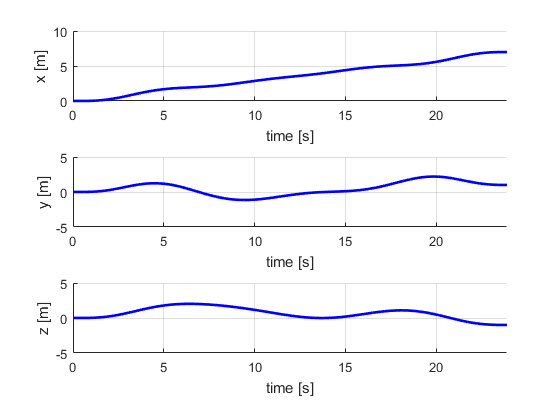
\includegraphics[width=3.5in]{images/quadposition.png}%
\label{fig_first_case}}
\hfil
\subfloat[]{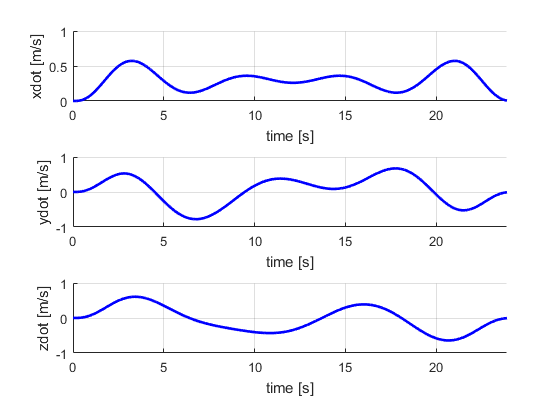
\includegraphics[width=3.5in]{images/quadvelocity.png}%
\label{fig_second_case}}
\caption{Position and velocity trajectories for quadrotor based on minimum snap. All the trajectories are smooth and based on differential flatness.}
\label{fig_sim}
\end{figure*} 

\begin{figure*}[htpb]
\centering
\subfloat[]{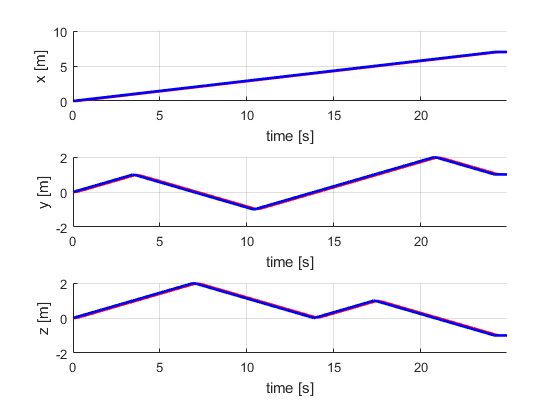
\includegraphics[width=3.5in]{images/quadpositionB.png}%
\label{fig_first_case1}}
\hfil
\subfloat[]{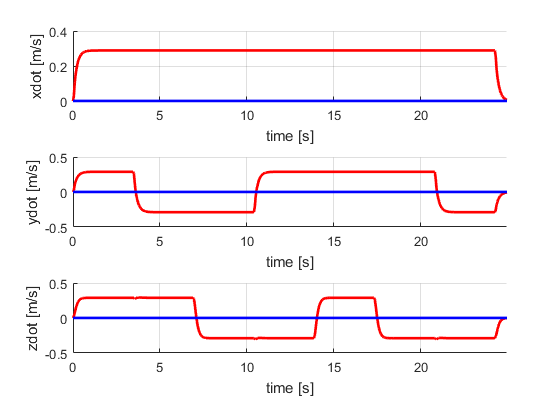
\includegraphics[width=3.5in]{images/quadvelocityB.png}%
\label{fig_second_case1}}
\caption{Position and velocity trajectories for quadrotor without minimum snap. The points are connected as linearly with each other based on shortest distance (minimum velocity).}
\label{fig_sim1}
\end{figure*}

\FloatBarrier
As we can observe from the \ref{fig_sim}, that the trajectories are smooth and there is no discontinuity in the system. The smooth trajectories allows better performance and planning of quadrotor. However, in \ref{fig_sim1}, it can be observed that the trajectories are not continuous, it passes through specified waypoints but because of sudden jump in the velocity and position graphs it's not smooth. Also, because of inertia present in the system, it may not be feasible to make such sharp turn.

%\begin{figure}[h!]
%\centering
%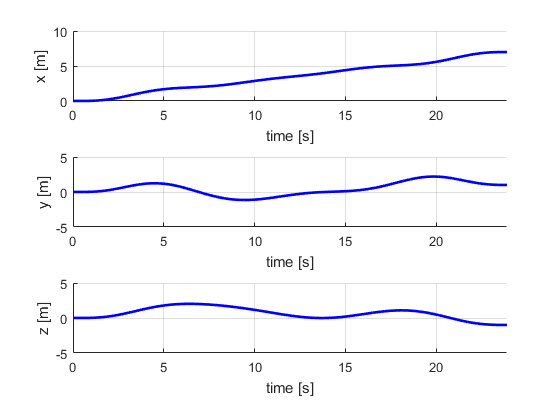
\includegraphics[scale=0.75]{images/quadposition.png}
%\caption{Quadrotor position trajectories.}
%\label{QuadposA}
%\end{figure}

%\begin{figure}[h!]
%\centering
%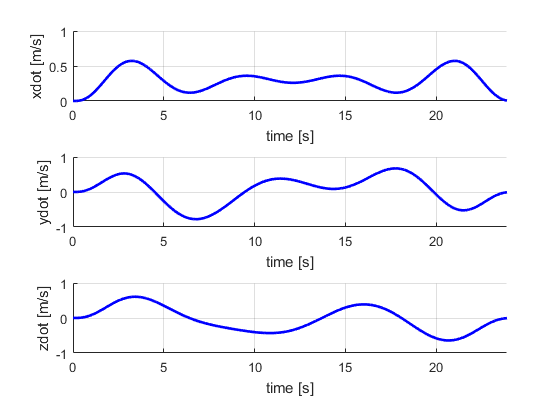
\includegraphics[scale=0.75]{images/quadvelocity.png}
%\caption{Quadrotor velocity trajectories.}
%\label{QuadvelA}
%\end{figure}
%\section{Conclusion}


\section{Conclusion}
From this project I learned interesting application of trajectory generation for quadrotors. Minimum snap trajectories can be used for aggressive maneuvers and perching and still system will have no any perturbations. This is one of the important concept, I learned from this project. The trajectories are always smooth and optimal. One can selected waypoints and introduce more dynamic behavior to the quadrotor. I plan to use differential flatness based trajectory generation for my future work and test in the experimental platform with one of our rotors. I also plan to extend it to multi-agents motion planning and control. 


%
%% conference papers do not normally have an appendix
%\appendices
%\section{Trajectory Generation Code}
%\section{Control Design}
%Appendix one text goes here.
%
%% you can choose not to have a title for an appendix
%% if you want by leaving the argument blank
%\section{}
%Appendix two text goes here.
%
%
%
%% use section* for acknowledgment
%\section*{Acknowledgment}


%The authors would like to thank..





% trigger a \newpage just before the given reference
% number - used to balance the columns on the last page
% adjust value as needed - may need to be readjusted if
% the document is modified later
%\IEEEtriggeratref{8}
% The "triggered" command can be changed if desired:
%\IEEEtriggercmd{\enlargethispage{-5in}}

% references section

% can use a bibliography generated by BibTeX as a .bbl file
% BibTeX documentation can be easily obtained at:
% http://mirror.ctan.org/biblio/bibtex/contrib/doc/
% The IEEEtran BibTeX style support page is at:
% http://www.michaelshell.org/tex/ieeetran/bibtex/
%\bibliographystyle{IEEEtran}
% argument is your BibTeX string definitions and bibliography database(s)
%\bibliography{IEEEabrv,../bib/paper}
%
% <OR> manually copy in the resultant .bbl file
% set second argument of \begin to the number of references
% (used to reserve space for the reference number labels box)
%\begin{thebibliography}{1}

%\bibitem{IEEEhowto:kopka}
%
%H.~Kopka and P.~W. Daly, \emph{A Guide to \LaTeX}, 3rd~ed.\hskip 1em plus
%  0.5em minus 0.4em\relax Harlow, England: Addison-Wesley, 1999.


\bibliographystyle{IEEEtran}
\bibliography{IEEEabrv,mybib}

%\end{thebibliography}




% that's all folks
\end{document}


